%% ma: L12-B13-0017
%% lop: 12
%% chuong: 4
%% bai: 13
%% dang: 12.13.1
%% loai: TLN
%% muc: VD
%% dap_an: "30"
%% nguon: "(NBV)-ĐỀ SỐ 6-MỖI NGÀY 1 ĐỀ THI 2025.pdf (D06, MỖI NGÀY 1 ĐỀ - Đề số 6), Phần III Câu 5"
%% kien_thuc: "Bài 13 (thể tích khối tròn xoay sinh bởi hình phẳng quay quanh trục Ox), Bài 12 (tích phân), phương trình đường tròn (lớp 10)"
%% trang_thai: chinh-thuc
%% ghi_chu: "Trùng ý tưởng với dạng 12.13.1 (thể tích khối tròn xoay) nên nhập cùng dạng. Đáp án gốc 30 đúng (V=28672π/3 cm3≈30025 cm3≈30 dm3, kiểm bằng sympy). Hình dựng lại bằng TikZ theo đề"
\begin{ex}
Họa sĩ thiết kế một chiếc mũ xe máy có dạng khối tròn xoay, mặt cắt đứng chứa tâm của khối tròn xoay có dạng một cung tròn bán kính $20$ cm, với độ dài dây cung là $32$ cm (hình bên). Thể tích của khối tròn xoay này là bao nhiêu $\text{dm}^3$? (Làm tròn kết quả đến hàng đơn vị)
\begin{center}
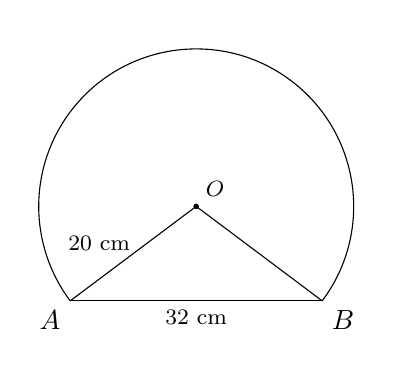
\begin{tikzpicture}[scale=1]
  \def\R{2}\def\h{1.2}\def\w{1.6}
  \draw (\w,-\h) arc[start angle=-36.87,end angle=216.87,radius=\R];
  \draw (-\w,-\h)--(\w,-\h);
  \draw (-\w,-\h)--(0,0)--(\w,-\h);
  \fill (0,0) circle (1pt);
  \path (0,0) node[above right,font=\footnotesize]{$O$} (-\w,-\h) node[below left]{$A$} (\w,-\h) node[below right]{$B$};
  \path (-.8,-.6) node[above left,font=\footnotesize,inner sep=1pt]{$20$ cm};
  \path (0,-\h) node[below,font=\footnotesize]{$32$ cm};
\end{tikzpicture}
\end{center}
\shortans{30}
\loigiai{Chọn hệ trục $Oxy$ có gốc $O$ là tâm đường tròn, trục $Ox$ là trục đối xứng của cung, đơn vị $1$ cm. Đường tròn có phương trình $x^2+y^2=400$. Gọi $H$ là trung điểm dây cung: $AH=16$ nên $OH=\sqrt{20^2-16^2}=12$, $H(-12;0)$.

Khối tròn xoay sinh bởi hình phẳng giới hạn bởi $y=\sqrt{400-x^2}$, trục $Ox$, $x=-12$, $x=20$ quay quanh $Ox$:
\[V=\pi\int_{-12}^{20}\left(400-x^2\right)\mathrm dx=\pi\left(400x-\dfrac{x^3}3\right)\Big|_{-12}^{20}=\dfrac{28672\pi}3\approx30\,025\ \text{cm}^3\approx30\ \text{dm}^3.\]}
\end{ex}
